	\documentclass[10pt,oneside]{CBFT_book}

	% Algunos paquetes
	\usepackage{amsmath}
	\usepackage{amssymb}
	\usepackage{graphicx}
	\usepackage{libertine}
	\usepackage{lipsum}
	\usepackage[numbers]{natbib}
	\setcitestyle{square}


	\usepackage{polyglossia}
	\setdefaultlanguage{spanish}

	\usepackage{CBFT.estilo} % Cargo la hoja de estilo


	% Tipografías
	% \setromanfont[Mapping=tex-text]{Linux Libertine O}
	% \setsansfont[Mapping=tex-text]{DejaVu Sans}
	% \setmonofont[Mapping=tex-text]{DejaVu Sans Mono}

	%===================================================================
	%	DOCUMENTO PROPIAMENTE DICHO
	%===================================================================

% \title{CBFT Mecánica clásica}
% \author{Mecánica lagrangiana}
% \date{\today}

\begin{document}
% \maketitle
% \tableofcontents
\chapter{Descripción de sistemas mecánicos}



% =================================================================================================
\section{Velocidad y aceleración en coordenadas cilíndricas y esféricas}
% =================================================================================================

En la resolución de los problemas dinámicos que surgen de las ecuaciones de Newton la igualdad vectorial involucrada debe,
en general, escribirse en algún sistema de coordenadas apropiado.
Esto implica para la aceleración la doble derivada con respecto al tiempo del vector de posición $ \vb{x}(t) $ en las
coordenadas en las cuales se halle escrito.

Obviando el sistema cartesiano rectangular usual $(x,y,z)$, los dos sistemas de coordenadas más sencillos son el de
coordenadas cilíndricas $(r,\varphi,z)$ y el de coordenadas esféricas $(r,\theta,\varphi)$. Los problemas más sencillos
de la dinámica implican geometrías donde estos sistemas son apropiados. Asimismo, muchas geometrías más complejas pueden
quizás en primera aproximación modelarse con estas coordenadas.

Así, por ejemplo, un vector genérico en términos de la base de versores cilíndricos $(\hat{r},\hat{\varphi},\hat{z})$ será
\[
	\vb{V}(t) = r \hat{r} + \varphi \hat{\varphi} + z \hat{z},
\]
de manera que su derivada con respecto al tiempo implica la derivación de cada coordenada y cada versor.

La gran ventaja de las coordenadas cartesianas es que los versores $ \hat{ x }, \hat{ y }, \hat{ z }$ tienen su orientación
constante para cualquier punto del espacio, razón por la cual no varían con el tiempo. Entonces, en general, resulta
conveniente evaluar las derivadas de los versores que sí varían con el tiempo (como por ejemplo $\hat{r}$) en términos de
su descomposición en cartesianas, puesto que sólo hay que derivar el coeficiente que lo acompaña.

Para coordenadas cartesianas, las fórmulas de velocidad y aceleración son triviales. A partir del vector de posición
\[
	\vb{x}(t) = x \hat{x} + y \hat{y}  + z\hat{z},
\]
se tienen
\[
	\vb{v}(t) \equiv \dtot{\vb{x}}{t}(t) = \dot{\vb{x}}(t) = \dot{x} \hat{x} + \dot{y} \hat{y}  + \dot{z}\hat{z},
\]
\[
	\vb{a}(t) \equiv \dtot[2]{\vb{x}}{t}(t) = \ddot{\vb{x}}(t) = \ddot{x} \hat{x} + \ddot{y} \hat{y}  + \ddot{z} \hat{z},
\]
donde con el objeto de no sobrecargar la notación no se ha explicitado la dependencia temporal en las coordenadas.

A continuación se deducen las fórmulas de velocidad y aceleración para las coordenadas cilíndricas y esféricas a partir de
un vector de posición $ \vb{x}(t) $ del origen\footnote{Un vector del origen tiene su base anclada en el origen del sistema
de coordenadas lo que causa que no tenga componentes angulares en los sistemas cilíndrico y esférico. Esta simplificación
es importante y en realidad si no fuera aplicable la utilización de estos sistemas tal vez pierda su razón de ser.}.


\subsection{Coordenadas cilíndricas}

% La gran ventaja de las coordenadas cartesianas es que los versores $ \hat{i}, \hat{j}, \hat{k}$ no varían con el tiempo,
% entonces
% \[
% 	\vb{r}(t) = x \hat{i} + y \hat{j}
% \]
% lleva a que
% \[
% 	\vb{v} = \dtot{\vb{r}}{t} = \dot{x}\hat{i} + \dot{y}\hat{j}
% \]
Un vector de posición del origen es
\[
	\vb{x}(t) = r \:\hat{r} + z \:\hat{z},
\]
y la derivada temporal se hace con la regla de Leibniz en el caso del primer término de la derecha,
\[
	\dtot{\vb{x}}{t} = \dtot{r}{t} \:\hat{r} + r \:\dtot{\hat{r}}{t} + \dtot{z}{t} \hat{z}
\]
y para evaluar la derivada temporal del versor consideramos la descomposición
\[
	\hat{r} = \cos \varphi \:\hat{x} + \sin \varphi \:\hat{y}
\]
\notamargen{
% \begin{figure}[h]
% 	\begin{center}
	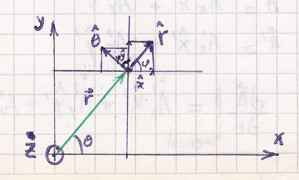
\includegraphics[scale=0.35]{images/fig_mc_polares_decomp.jpg}
% 	\end{center}
% 	\caption{}
% \end{figure}
}
\[
	\hat{\varphi} = -\sin \varphi  \:\hat{x} + \cos  \varphi \:\hat{y}
\]
que lleva a
\[
	\dtot{\hat{r}}{t} = - \sin \varphi \: \dot{ \varphi } \:\hat{x} + \cos \varphi \: \dot{ \varphi } \:\hat{y} =
	\dot{\vp} \: \hat{\vp}
\]
y entonces
\[
	\dtot{\vb{x}}{t} = \dot{r} \:\hat{r } + r \:\dot{\vp} \: \hat{\vp} + \dot{z} \:\hat{z}.
\]

\notamargen{
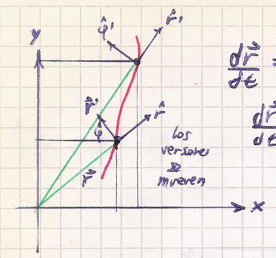
\includegraphics[scale=0.4]{images/fig_mc_polares_arbitrario.jpg}
}
% que se puede escribir como
% \[
% 	\dtot{\vb{r}}{t} = \dot{r} \: \hat{r } + r \dot{\vp} \: \hat{\vp} = \dot{\vb{r}}
% \]
% y extraemos de conclusión que
% \[
% 	\dtot{\hat{r}}{t} = \dot{\vp} \: \hat{\vp}
% \]

Para la aceleración hay que derivar la velocidad con respecto al tiempo
\[
	\ddot{\vb{x}} = \dtot{}{t} ( \dot{r} \: \hat{r} + r\dot{\vp} \: \hat{\vp} + \dot{z} \:\hat{z} )
\]
\[
	\ddot{\vb{x}} = \ddot{r} \:\hat{r} + \dot{r} \: \dtot{\hat{r}}{t} + \dot{r} \: \dot{\vp} \: \hat{\vp}
	+ r \left( \ddot{\vp} \: \phiver + \dot{\vp} \: \dtot{\hat{\vp}}{t} \right) + \ddot{z} \:\hat{z}
\]
y utilizando
\[
	\dtot{\hat{\vp}}{t} = - \dot{ \vp } ( \cos \vp \:\hat{x} + \sin  \vp \:\hat{y} ) = - \dot{\vp} \: \hat{r}
\]
finalmente se arriba a
\[
	\ddot{\vb{x}} = ( \ddot{r} - r\dot{\vp}^2 ) \rver + ( r\ddot{\vp} + 2 \dot{r} \dot{\vp} ) \phiver + \ddot{z} \:\hat{z}.
\]

Para problemas de dos dimensiones suele utilizarse un sistema coordenado, conocido como coordenadas polares, que es el
de cilíndricas con $ z \equiv 0 $. Las expresiones de velocidad y aceleración polares correspondientes serán las
obtenidas en esta sección luego de {\it borrar} la coordenada $z$.

\subsection{Coordenadas esféricas}

Para el sistema esférico la deducción de la equivalencia cartesiana de los versores es un poco más trabajosa que en el
sistema cilíndrico (donde en realidad estos versores viven en un plano $z$ cte.) y el álgebra implicado es algo
engorroso. La expresión de los versores es
\[
	\rver = \cos\vp \sin\theta\xver + \sin\vp\sin\theta\yver + \cos\theta\zver,
\]
\[
	\phiver = -\sin\vp \xver + \cos\vp \yver,
\]
\[
	\thetaver = \cos\theta \cos\vp \xver + \cos\theta\sin\vp\yver - \sin\theta\zver.
\]
\notamargen{Dado que este es un curso básico pero que se jacta de visual, tendriamos que poner ilustraciones del
carajo de los vectores en esféricas y cilíndricas para que quede intuitivo sus dificultades cuando el problema en
cuestión no tiene las simetrías explícitas de estos sistemas.}

Un vector de posición es simplemente
\[
	\vb{x} = r \rver
\]
aunque en el $\rver$ está {\it escondida} la dependencia angular. Consignaremos a continuación solamente las
expresiones finales para la velocidad y aceleración, que son respectivamente
\[
	\vb{v} = \dot{\vb{x}} = \dot{r} \rver + r\dot{\theta}\thetaver + r\dot{\vp}\sin\theta\phiver
\]
\begin{multline*} % \vb no se da cuenta que multline ES modo matemático (por ello el .\ inicial)
	\!\: \vb{a} = \ddot{\vb{x}} = ( \ddot{r} - r\dot{\theta}^2 - r\dot{\vp}^2 \sin^2 \theta )\rver +
	( r\ddot{\theta} + 2\dot{r}\dot{\theta} - r\dot{\vp}^2 \sin \theta \cos\theta )\thetaver \: + \\
	( r \ddot{\vp}\sin\theta + 2 \: \dot{r} \: \dot{\vp} \sin\theta + 2 \: r \:\dot{\theta} \:\dot{\vp} \cos\theta )\phiver
\end{multline*}


% =================================================================================================
\section{Transformación entre sistemas en rotación}
% =================================================================================================

Otro tipo de transformación común entre sistemas de coordenadas (en el plano) que comparten origen es la rotación.

Suponiendo un sistema de coordenadas $(x,y)$ fijo (que llamaremos ``inercial'') de origen $O$ y otro de coordenadas
$(x',y')$, que está rotando en torno a ese origen (sistema ``móvil''), interesa ver qué consecuencias tiene sobre la
velocidad y aceleración de un vector de posición \vb{A}, el hecho de determinarlas desde uno u otro sistema. Si bien
hablamos de un sistema {\it fijo}, en realidad ambos se hallan en rotación entre sí.

Como se ve en la FIGURA XXX
\notamargen{
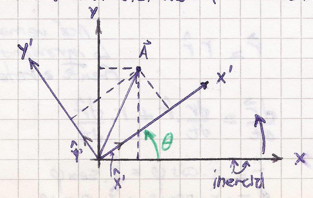
\includegraphics[scale=0.4]{images/fig_mc_sist_rotantes.jpg}
}
la posición instantánea entre sistemas está determinada por el ángulo $\theta(t)$ y, dado que ambos sistemas comparten
el origen, los mismos son coincidentes en $\theta = 0$.
% Como el sistema en rotación varía la posición de sus ejes con el tiempo, sus versores asociados $(\xver', \yver')$
% también variarán con el tiempo (pese a que son cartesianos).

Dado que los sistemas no se hallan entre sí a velocidad constante\footnote{Aún en el caso de $ \theta(t) = cte.$ la
velocidad no es constante como vector puesto que cambia de dirección todo el tiempo.} es patente que las ecuaciones de
Newton se verán modificadas.
Para un vector \vb{A} constante con respecto al sistema inercial, cualitativamente esperaríamos observarlo desde el
sistema móvil en alguna suerte de movimiento dado por el efecto dinámico de la rotación\footnote{Si estoy montado en el
caballo de madera de una calesita veré a mi abuela, que me espera inmóvil a un lado, como dotada de movimiento.}. Veamos
qué surge de la cuenta algebraica.

El mismo vector de acuerdo a los dos sistemas de coordenadas en el plano, es
\[
	\vb{A}(t) = A_x\xver + A_y\yver         \qquad\qquad               \vb{A}'(t) = A_x'\xver' + A_y'\yver'
\]
donde las coordenadas primadas refieren al sistema móvil. Nótese que los versores asociados en ambos casos $(\xver,
\yver)$ y $(\xver', \yver')$ son constantes, esto es, no dependen del tiempo. Que ambos sistemas se hallen en rotación
entre sí no es intrínseco de alguno de ellos.
Un observador del sistema primado ve a sus ejes fijos mientras que en las medidas que realiza sobre \vb{A} verá una
dinámica particular.

Si consideramos la variación temporal de \vb{A}' pero como es vista desde el sistema inercial resulta
\[
	\left. \dtot{\vb{A}}{t} \right|_\text{inercial} =
	\dot{A_x'} \xver' + A_x'\dot{\xver'} + \dot{A_y'}\yver' + A_y' \dot{\yver'},
\]
porque para un observador en el sistema inercial se mueven las componentes del vector y los versores.

\notamargen{Esta notación es oscura, habría que ver una mejor manera de explicar esto.}

La variación temporal de los versores la conocemos porque es la misma situación geométrica que la encontrada para el
caso de los versores cilíndricos $(\rver,\phiver)$. Podemos hallar la equivalencia
\[
	\dtot{\hat{x}'}{t} = \dot{\theta} \yver'         \qquad \qquad          \dtot{\hat{y}'}{t} = -\dot{\theta} \xver'.
\]

Desde el sistema móvil los versores son por supuesto constantes (el sistema móvil no es consciente de su movimiento) de
modo que
\[
	\left. \dtot{\vb{A}}{t} \right|_\text{móvil} = \dot{A_x'}\xver' + \dot{A_y'}\yver'
\]
y entonces
\[
	\left. \dtot{\vb{A}}{t} \right|_\text{fijo} = \left. \dtot{\vb{A}}{t} \right|_\text{móvil}
	+ A_x' \dot{\theta}\yver' - A_y'\dot{\theta}\xver'.
\]
% donde
% \[
% 	\left. \dtot{\vb{A}'}{t} \right|_\text{móvil} \equiv \sum_i \dtot{A_i'}{t} \: \hat{e_i}'
% \]
% \[
% 	\left. \dtot{\vb{A}}{t} \right|_\text{móvil} = \dot{A_x'}\xver' + \dot{A_y'}\yver'
% \]

Si definimos
\[
	\vb{\omega} = \dot{\theta} \zver,
\]
entonces resulta que
\[
	\vb{\omega}\times\vb{A}' = \dot{\theta} \zver \times ({A_x'}\xver' + {A_y'}\yver') =
	A_x' \dot{\theta}\yver' - A_y'\dot{\theta}\xver'.
\]

Volviendo a la derivada de \vb{A} tenemos
\[
	\left. \dtot{\vb{A}}{t} \right|_\text{fijo} = \left. \dtot{\vb{A}}{t} \right|_\text{móvil}
	+ \vb{\omega} \times \vb{A}'
\]
que nos da la variación temporal de un vector \vb{A} visto desde un sistema fijo en términos de lo que se mediría
en un sistema (móvil) que está en rotación respecto al primero.

Si ahora la especializamos para un vector de posición \vb{x}, obtenemos la velocidad
\[
	\left. \vb{v} \right|_\text{fijo} = \left. \vb{v} \right|_\text{móvil} + \vb{\omega} \times \vb{x}',
\]
donde
\[
	\left. \vb{v} \right|_\text{móvil} = \dot{x}' \xver' + \dot{y}' \yver'
\]

Asimismo, la aceleración se obtiene aplicando la relación al vector $\vb{v} \equiv d\vb{x}/dt$, de manera que
tendremos
\[
	\left. \vb{a} \right|_\text{fijo} = \left. \dtot{\vb{v}}{t} \right|_\text{fijo} = \left. \dtot{\vb{v}}{t} \right|_\text{móvil} +
	\vb{\omega} \times \vb{v}'
\]
\[
	\left. \vb{a} \right|_\text{fijo} =
	\dtot{}{t}\left[ \left. \dtot{\vb{x}}{t} \right|_\text{móvil} + \vb{\omega}\times\vb{x}' \right] +
	\vb{\omega} \times \left[ \left. \vb{v} \right|_\text{móvil} +	\vb{\omega}\times\vb{x}' \right]
\]

Ahora procedemos a trabajar las expresiones dentro del primer corchete, empezando por la derivada temporal de la velocidad
en el sistema móvil,
\[
	\left. \vb{a} \right|_\text{móvil} \equiv
	\dtot{}{t}\left.( \dot{x}' \xver' + \dot{y}' \yver' )\right|_\text{móvil} = \ddot{x}' \xver' + \ddot{y}' \yver'
\]
y continuando con el término
\[
	\left.\vb{\omega}\times\vb{x}'\right|_\text{móvil} = \omega x' \yver' - \omega y' \xver' ,
\]
cuya derivada es
\[
	\dtot{}{t}\left.\vb{\omega}\times\vb{x}\right|_\text{móvil} =
	-( \dot{\omega} y' + \omega \dot{y}' )\xver' + ( \dot{\omega} x' + \omega \dot{x}' )\yver' =
	\left. \vb{\omega} \times\vb{v}'\right|_\text{móvil} + \left.\dot{\vb{\omega}} \times\vb{x}'\right|_\text{móvil}
\]

Juntando todo resulta
\[
	\left. \vb{a}\right|_\text{fijo} = \left. \vb{a}\right|_\text{móvil}
	+ \left.\dot{\vb{\omega}} \times\vb{x}'\right|_\text{móvil} + 2 \:\vb{\omega}\times\vb{v'} + \vb{\omega}
	\times (\vb{\omega} \times \vb{x}')
\]
donde el tercero es la aceleración de Coriolis y el cuarto la aceleración centrípeta.

Las leyes de Newton observadas desde el sistema fijo serán
% Llamando $ \alpha = \dot{\omega} = \dtot{\omega}{t}$ resulta
\[
	\vb{F} = m\vb{a} = m \left. \vb{a}\right|_\text{móvil} + m \: \dot{ \vb{\omega} } \times \vb{r} + 4 \: m \:
	\vb{\omega}\times\vb{v'} + m \: [  \vb{\omega} \times (\vb{\omega}\times\vb{r} )]
\]
que se pueden reacomodar como
\[
	m \left. \vb{a}\right|_\text{fijo} =
	\vb{F} - m \left. \vb{a}\right|_\text{móvil} - m \: \dot{\vb{\omega}} \times \vb{r} - 4 \: m \: \vb{\omega}\times\vb{v'} -
	m \: [\vb{\omega} \times(\vb{\omega}\times\vb{r})]
\]
donde ahora en el RHS tenemos la fuerza $\vb{F}$ que es la única que produce par de acción y reacción, y los términos de
fuerza lineal, de Coriolis y centrífuga.

Si $\vb{\omega} = cte.$ entonces la fuerza lineal es nula.

\notamargen{Está un poco inconsistente la notación utilizada, con lo de móvil y la prima. La carpeta tiene muchos
typos. El 'Problema' de la hoja 5R no lo entiendo; en realidad parece estar vinculado a sólidos. Habría que decidir si
ponerlo o no. En caso negativo, ¿qué otro se puede ubicar?}


% ============================================================================

% \bibliographystyle{CBFT-apa-good} % (uses file "apa-good.bst")
% \bibliography{CBFT.Referencias} % La base de datos bibliográfica


\end{document}
